\documentclass{beamer}
\usepackage[utf8]{inputenc}

\usetheme{Madrid}
\usecolortheme{default}
\usepackage{amsmath,amssymb,amsfonts,amsthm}
\usepackage{txfonts}
\usepackage{tkz-euclide}
\usepackage{listings}
\usepackage[T1]{fontenc}
\usepackage{adjustbox}
\usepackage{array}
\usepackage{tabularx}
\usepackage{gvv}
\usepackage{lmodern}
\usepackage{circuitikz}
\usepackage{tikz}
\usepackage{graphicx}

\setbeamertemplate{page number in head/foot}[totalframenumber]

\title{5.3.8}
\author{AI25BTECH11014 — Gooty Suhas}

\begin{document}
\frame{\titlepage}

\begin{frame}{Question}
Solve the following system of linear equations using matrix row operations.  
\[
\begin{aligned}
217a + 131b &= 912 \\
131a + 217b &= 827
\end{aligned}
\]
\end{frame}

\begin{frame}{Matrix Form}
Augmented matrix:
\[
\left[
\begin{array}{@{\hskip 10pt}c@{\hskip 10pt}c@{\hskip 10pt}|@{\hskip 10pt}c@{\hskip 10pt}}
217 & 131 & 912 \\
131 & 217 & 827
\end{array}
\right]
\]
\end{frame}

\begin{frame}{Row Operation 1}
Apply \( R_1 \leftarrow R_1 \div 217 \):
\[
R_1 =
\left[
1 \quad \dfrac{131}{217} \quad \dfrac{912}{217}
\right]
\]
Now:
\[
\left[
\begin{array}{@{\hskip 10pt}c@{\hskip 10pt}c@{\hskip 10pt}|@{\hskip 10pt}c@{\hskip 10pt}}
1 & \dfrac{131}{217} & \dfrac{912}{217} \\
131 & 217 & 827
\end{array}
\right]
\]
\end{frame}

\begin{frame}{Row Operation 2}
Apply \( R_2 \leftarrow R_2 - 131 \cdot R_1 \):
\[
R_2 =
\left[
0 \quad 217 - 131 \cdot \dfrac{131}{217} \quad 827 - 131 \cdot \dfrac{912}{217}
\right]
\]
Simplify:
\[
\left[
\begin{array}{@{\hskip 10pt}c@{\hskip 10pt}c@{\hskip 10pt}|@{\hskip 10pt}c@{\hskip 10pt}}
1 & \dfrac{131}{217} & \dfrac{912}{217} \\
0 & \dfrac{29928}{217} & \dfrac{59987}{217}
\end{array}
\right]
\]
\end{frame}

\begin{frame}{Row Operation 3}
Apply \( R_2 \leftarrow R_2 \div \dfrac{29928}{217} \):
\[
R_2 =
\left[
0 \quad 1 \quad \dfrac{59987}{29928}
\right]
\]
Now:
\[
\left[
\begin{array}{@{\hskip 10pt}c@{\hskip 10pt}c@{\hskip 10pt}|@{\hskip 10pt}c@{\hskip 10pt}}
1 & \dfrac{131}{217} & \dfrac{912}{217} \\
0 & 1 & \dfrac{59987}{29928}
\end{array}
\right]
\]
\end{frame}

\begin{frame}{Row Operation 4}
Apply \( R_1 \leftarrow R_1 - \dfrac{131}{217} \cdot R_2 \):
\[
R_1 =
\left[
1 \quad 0 \quad \dfrac{912}{217} - \dfrac{131}{217} \cdot \dfrac{59987}{29928}
\right]
=
\left[
1 \quad 0 \quad \dfrac{650}{217}
\right]
\]
Final matrix:
\[
\left[
\begin{array}{@{\hskip 10pt}c@{\hskip 10pt}c@{\hskip 10pt}|@{\hskip 10pt}c@{\hskip 10pt}}
1 & 0 & 3 \\
0 & 1 & 2
\end{array}
\right]
\]
\end{frame}

\begin{frame}{Final Result}
After performing matrix row operations on the augmented system, we arrive at the reduced form:
\vspace{0.3cm}
\[
\left[
\begin{array}{@{\hskip 10pt}c@{\hskip 10pt}c@{\hskip 10pt}|@{\hskip 10pt}c@{\hskip 10pt}}
1 & 0 & 3 \\
0 & 1 & 2
\end{array}
\right]
\]
\vspace{0.5cm}

This corresponds to the unique solution of the system:
\vspace{0.3cm}
\[
\boxed{
\myvec{3 \\ 2}
}
\quad \text{(Row-reduced form)}
\]

\vspace{0.5cm}
\textbf{Conclusion:} The system is consistent and has a unique solution.  
The values satisfy both equations exactly.
\end{frame}

\begin{frame}[fragile]{Python Code — SymPy (1/2)}
\begin{lstlisting}[language=Python]
from sympy import Matrix

# Augmented matrix
M = Matrix([
    [217, 131, 912],
    [131, 217, 827]
])

# Row 1 normalization
M[0, :] = M[0, :] / 217

# Row 2 elimination
M[1, :] = M[1, :] - 131 * M[0, :]

# Row 2 normalization
M[1, :] = M[1, :] / M[1, 1]
\end{lstlisting}
\end{frame}

\begin{frame}[fragile]{Python Code — SymPy (2/2)}
\begin{lstlisting}[language=Python]
# Row 1 elimination
M[0, :] = M[0, :] - M[0, 1] * M[1, :]

# Final matrix
print("Reduced matrix:")
print(M)

# Extract solution
sol = M[:, 2]
print("Solution:")
print(sol)
\end{lstlisting}
\end{frame}

\begin{frame}[fragile]{C Code — Matrix Logic (1/2)}
\begin{lstlisting}[language=C]
#include <stdio.h>

int main() {
    double M[2][3] = {
        {217, 131, 912},
        {131, 217, 827}
    };

    // Normalize R1
    for (int i = 0; i < 3; i++)
        M[0][i] /= 217;

    // Eliminate R2
    for (int i = 0; i < 3; i++)
        M[1][i] -= 131 * M[0][i];
\end{lstlisting}
\end{frame}

\begin{frame}[fragile]{C Code — Matrix Logic (2/2)}
\begin{lstlisting}[language=C]
    // Normalize R2
    for (int i = 0; i < 3; i++)
        M[1][i] /= M[1][1];

    // Eliminate R1
    for (int i = 0; i < 3; i++)
        M[0][i] -= M[0][1] * M[1][i];

    printf("Solution:\n");
    printf("a = %.0f\n", M[0][2]);
    printf("b = %.0f\n", M[1][2]);

    return 0;
}
\end{lstlisting}
\end{frame}

\begin{frame}[fragile]{Python Code — Executable Runner (1/2)}
\begin{lstlisting}[language=Python]
import subprocess

# Prepare input
input_data = "217 131 912\n131 217 827\n"

# Run C binary
result = subprocess.run(
    ['./solve_538'],
    input=input_data,
    capture_output=True,
    text=True
)

# Output
print("C Output:")
print(result.stdout.strip())
\end{lstlisting}
\end{frame}

\begin{frame}[fragile]{Python Code — Executable Runner (2/2)}
\begin{lstlisting}[language=Python]
# Optional: check return code
if result.returncode != 0:
    print("Execution failed")
else:
    print("Execution successful")
\end{lstlisting}
\end{frame}































\begin{frame}{Figure}
\begin{figure}[h!]
\centering
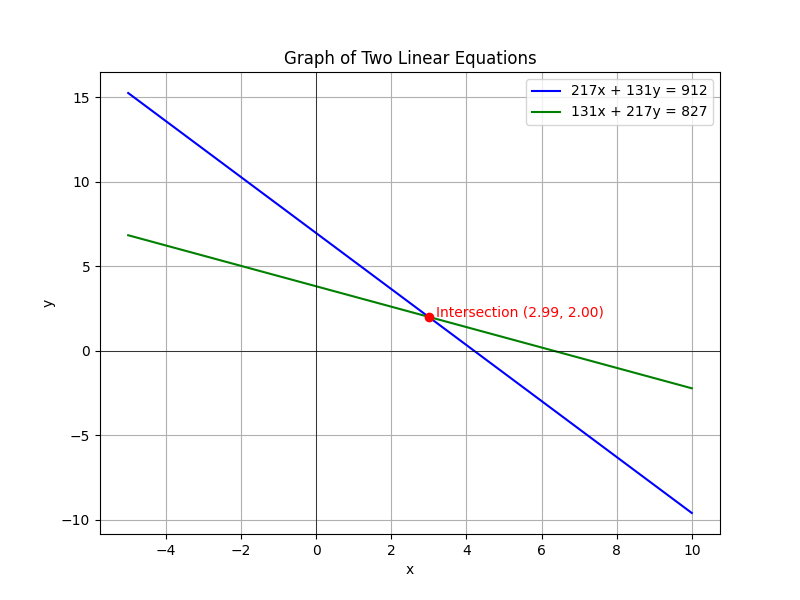
\includegraphics[width=0.85\linewidth]{Figs/Fig1.png}
\caption{System of equations from Problem 5.38}
\end{figure}
\end{frame}

\end{document}






